\chapter{文脈を考慮した言語特徴量の検討}

\section{文脈を考慮した言語特徴量}

% 前後が役に立つことは分かっている.南条
% 金沢の人文献
% 周囲の言語を含めた特徴量を含めた

% TODO: 参考文献 音響学会15 金寺
NTCIR11 SpokenQuery\&Doc Formal-run の SQSCR SGS Retrieval条件では,検索対象の文書に対し,周囲の文書を利用すると検索精度が向上する事を報告している.
% 金寺ら\cite{kanetera}は音声内容検索において,検索対象文書の周囲に存在する文書に対し,シーンべクトルの線形補間を用いて音声情報検索を行った結果,検索性能が高いことが報告されている. 
Nanjoら\cite{nanjo}は,検索対象を15発話単位, 30発話単位, 60発話単位, 全体の重み付き線形和によって検索べクトルを構成し, 検索精度に対し,良好な結果を得ている.
そこで本研究では,クエリ尤度を用いた検索モデルに対し,検索対象の周囲の単語を考慮することで,検索精度を改善する事を考案する.

% クエリ尤度と拡張
% 参考: http://www.fit.vutbr.cz/~imikolov/rnnlm/is2011_emp.pdf
% クエリ尤度モデルにおいて,零確率問題を回避するために,式(\ref{eq_dirichlet})を用いて,ディリクレスムージングを行う.この式(\ref{eq_dirichlet})の文書コレクションから推定されたモデル $\theta_C$ と共に,周囲の単語の特徴量を付与することで,検索対象文書に適切な文書コレクションでスムージングを行い,検索性能を高める. 
% 周囲の単語の特徴量 $P(w_i|h)$ を追加したときの, 式を式(\ref{eq_expanddirichlet_context})に示す.

% \begin{flalign}
%     & P(w_i|\theta_C; \mu; \nu) = \nonumber \\ 
%     & \frac{|D|}{|D|+\mu+\nu}\frac{c(w_i, D)}{|D|} + \frac{\mu}{|D|+\mu+\nu}P(w_i|\theta_C) & \nonumber \\
%     & + \frac{\nu}{|D|+\mu+\nu}P(w_i|h) 
%     \label{eq_expanddirichlet_context}
% \end{flalign}

% TODO: コーパスに文書コレクションと同様にプラスαする事を説明する
% TODO: 参考論文
% 本研究では,$P(w_i|h)$ を推定するための文書モデルとして,キャッシュモデル・N-gram言語モデル・リカレントニューラルネットワーク言語モデルを検討する.Mikolovら\cite{mikolov}は,キャッシュモデル・N-gram言語モデル(Kneser-Neyスムージング)・リカレントニューラルネットワークモデルを用い,言語モデルを構築する事で言語モデルの評価基準であるパープレキシティを減少させることに成功している.そのため,本研究でも,言語特徴量として有効であると推察できるキャッシュモデル・N-gram言語モデル・リカレントニューラルネットワーク言語モデルの3つモデルを用いる事で,検索精度がどのように変化するかを分析する.

Mikolovら\cite{mikolov}は,キャッシュモデル・N-gram言語モデル(Kneser-Neyスムージング)・リカレントニューラルネットワークモデルを用い,言語モデルを構築する事で言語モデルの評価基準であるパープレキシティを減少させることに成功している.そのため,本研究でも,言語特徴量として有効であると推察できるキャッシュモデル・N-gram言語モデル・リカレントニューラルネットワーク言語モデルの3つモデルをクエリ尤度モデルに用いる事で,検索精度がどのように変化するかを分析する.

% 参考: http://www.ar.media.kyoto-u.ac.jp/lab/bib/report/NEM-sdp07.pdf
\section{キャッシュモデル}
キャッシュモデルでは,単語 $w_n$ の直前の単語履歴をキャッシュ $H = \{ w_{n-|H|}, ..., w_{n-1}\} $ として記憶し,これに含まれる単語が再び使用される確率が高いと予測する.このキャッシュに基づく単語 $w_n$ の出現確率 $P_c(w_n|H)$ は式(\ref{cache})によって与えられる. ただし,$|H|$ は単語履歴 $H$ の長さ, $\delta$ はクロネッカーのデルタ関数である.

\begin{equation}
		P_c(w_n|H) = \frac{1}{|H|} \sum_{w_h \in H} \delta (w_n, w_h)
    \label{cache}
\end{equation}

本研究では,クエリ尤度モデルの式(\ref{eq_dirichlet2})の第1項 $\frac{c(w_i, d)}{|d|}$ とキャッシュモデル $P_c(w_n|H)$ を線形補間することにより,検索対象の周囲の単語を考慮し,検索精度の向上を図る.キャッシュモデルを適用したクエリ尤度モデルの式を式(\ref{eq_dirichlet_cache})に示す.ここで $\alpha$ はハイパーパラメーターである.

\begin{equation}
\begin{split}
    P(w_i|\theta_d;\mu) = \frac{|d|}{|d|+\mu} \Biggl( \gamma \frac{c(w_i, d)}{|d|} + (1 - \gamma) P_c(w_n|H) \Biggr)\\
    + \frac{\mu}{|d|+\mu} P(w_i|\theta_C)  
    \label{eq_dirichlet_cache}
\end{split}
\end{equation}

% 参考: http://www.cl.cs.titech.ac.jp/~fujii/paper/asj2002akiba.pdf
\section{N-gramとスムージング}
\subsection{概要}
式(\ref{eq_unigram2})で示した,ユニグラム言語モデルに基づくクエリ尤度モデルの拡張を考えるとき,直感的に,N-gram言語モデルへの展開が考えられる.例として,バイグラムに基づくクエリ尤度は式(\ref{ngram_like})で与えられる.\cite{bigram}

\begin{equation}
\begin{split}
    P(Q|\theta_D) = \prod_{i=1}^{|Q|} P(q_i|q^{i-1}_{1}, \theta_D) \\
    = P(q_1, \theta_D) \prod_{i=2}^{|Q|} P(q_i|q_{i-1}, \theta_D)
    \label{ngram_like}
\end{split}
\end{equation}

$P(q_i|q_i, \theta_D)$ は文書 $D$ のもとで $q_{i-1}$ の直後にクエリ語 $q_i$ が生成される確率である.本研究では,式(\ref{ngram_like})と同様に,N-gram言語モデルをクエリ尤度モデルに適用し,ディリクレスムージングを行なう.N-gram言語モデルをクエリ尤度モデルに適用した式を式(\ref{eq_dirichlet_ngram})に示す.

\begin{equation}
\begin{split}
    P(w_i|\theta_d;\mu) = \frac{|d|}{|d|+\mu} P(w_i|w^{i-1}_{1}, \theta_D)
    + \frac{\mu}{|d|+\mu} P(w_i|\theta_C)  
    \label{eq_dirichlet_ngram}
\end{split}
\end{equation}

N-gram言語モデルでは,学習データに現れない単語列を扱うため,種々の平滑化(スムージング)手法が適用される.スムージングの一つとして,バックオフ・スムージングでは,高次のN-gramが存在しない場合,低次のN-gramで代用する.

\subsection{単語連接を重視したバックオフ・スムージング}
バックオフ・スムージングの一般式は次のように表される.

\begin{equation}
		P(w_i|w_{i-n+1}^{i-1}) = 
    \begin{cases} 
        d_{w_{i-n+1}^i} P_{ML}(w_i|w_{i-n+1}^{i-1}) \\
        \hspace{\fill} (if\ C(w_{i-n+1}^{i-1}) > 0\ )\\ 
        \alpha(w_{i-n+1}^{i-1})P(w_i|w_{i-n+2}^{i-1})\\ 
        \hspace{\fill} (if\ C(w_{i-n+1}^{i-1}) = 0\ )
    \end{cases} 
    \label{ngram_smoosing1}
\end{equation}

ここで $d$, $P_{ML}$, $\alpha$は,それぞれ,ディスカウント係
数,最尤推定によるN-gram確率,確率の総和を1とするための正規化係数である.

\subsection{Kneser-Ney スムージング}

% TODO: 使い方を明記
% TODO: 使い方を要検討・学習がdocのみなので,クエリ尤度的には正しいが...

KneserとNey[3]は,絶対法[4]を拡張した平滑化手法を示している.
純粋に平滑化手法として他の手法と比べた場合でも,英語に適用した例で優れた性能を示すことが報告されている[2].Kneser-Neyスムージングでは,高次のN-gram確率が利用できない(信頼できない)場合に使用する低次の確率として,最尤推定による確率 $P_{ML} (w_i|w_{i-n+1}^{i-1})$ の代わりに次の値 $P_{KN} (w_i|w_{i-n+1}^{i-1})$ を用いる.

\begin{equation}
		P_{KN} (w_i|w_{i-n+1}) = \frac{|\{w_{i-n}|C(w_{i-n+1}^{i-1}) > 0\}|}{\sum_{w_i} |\{w_{i-n}|C(w_{i-n+1}^{i-1}) > 0\}|} 
    \label{ngram_smoosing2}
\end{equation}

ここで $|\{w_{i-n}|C(w_{i-n+1}^{i-1}) > 0\}|$ は, $w_{i-n}$ を変化させたときに,$C(w_{i-n+1}^{i-1})$ が0より大きいものの数の和である.
Kneser-Neyスムージングでは,長さ $N$ のN-gramについて, $n  <  N$ である全ての $n$ に対し,$P_{KN} (w_i|w_{i-n+1}^{i-1})$ を用いる.

% 参考: 複数の文脈長を考慮したリカレントニューラルネットワークに基づく言語モデル
\section{リカレントニューラルネットワーク}
リカレントニューラルネットワークに基づく言語モデル(RNNLM : Recurrent Neural Network Language Model)は,入力層 $\bm{w}$ ,潜在層 $\bm{s}$ ,出力層 $\bm{y}$ から構成されるニューラルネットワークに基づく言語モデルである.リカレントニューラルネットワークの構造を図\ref{fig_rnn}に示す.

\begin{figure}[h]
    \centering
    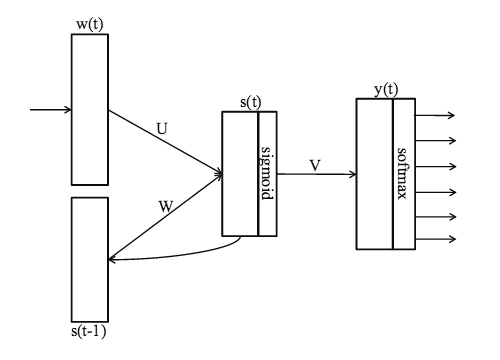
\includegraphics[width=7cm]{./image/rnn.png}
    \caption{リカレントニューラルネットワークの構造}
    \label{fig_rnn}
\end{figure}

リカレントニューラルネットワークは,潜在層 $\bm{s}$ に文脈を考慮するためのフィードバック構造をもつ. 潜在層 $s(t)$は,時刻 $t$ における単語の1-of-K表現 $w(t)$ と直前の時刻 $t−1$
の潜在層 $s(t−1)$ から成り,式(\ref{rnn1})で表される.

\begin{equation}
    s(t) = f(Uw(t) + Ws(t-1))
    \label{rnn1}
\end{equation}

ただし, $U$, $W$はそれぞれ入力層 $\bm{w}$ と潜在層 $\bm{s}$との間の重みパラメータ,潜在層 $s(t)$ と $s(t-1)$との間の重みパラメータ,$f(・)$ はシグモイド関数である.
入力 $w(t)$ は潜在層 $s(t)$ へ変換され,出力層 $y(t)$ で次の時刻 $t+1$ に現れる単語の生起確率が算出される.

\begin{equation}
		y(t) = g(Vs(t))
    \label{rnn3}
\end{equation}

ただし, $V$は潜在層 $\bm{s}$
と出力層 $\bm{y}$ との間の重みパラメータで, $g(・)$ はソフトマックス関数である.

% TODO: 参考文献 

リカレントニューラルネットワーク言語モデルは時刻 $t$ の次に予測すべき単語を教師信号としバックプロパゲーションによる学習を行う.特に,潜在層のフィードバック構造を時間方向に展開しバックプロパゲーションを行なうことで長期的な文脈情報を学習する.
% モデルの訓練方法の詳細については,[??,??]を参照されたい.

% TODO: 図とか必要な気がする
本研究では, まずNTCIR11のSpokenDocタスクで,提供されている講演文書に対してリカレントニューラルネットワーク言語モデルを用いて学習を行う.そして,講演文書内の検索対象となる文書までの単語をリカレントニューラルネットワーク言語モデルに入力することで,検索対象文書とそれまでの講演の内容を加味した,次の単語 $w_i$ の予測確率 $P(w_i|w_1^{i-1})$ を取得する.この$P(w_i|w_1^{i-1})$ を式(\ref{eq_dirichlet_cache})と同様に用い,クエリ尤度モデルに適用させる.リカレントニューラルネットワーク言語モデルを適用したクエリ尤度モデルを式(\ref{eq_dirichlet_rnn})に示す.

\begin{equation}
\begin{split}
    P(w_i|\theta_d;\mu) = \frac{|d|}{|d|+\mu} \Biggl( \gamma \frac{c(w_i, d)}{|d|} + (1 - \gamma) P(w_i|w_1^{i-1}) \Biggr)\\
    + \frac{\mu}{|d|+\mu} P(w_i|\theta_C)
    \label{eq_dirichlet_rnn}
\end{split}
\end{equation}


\section{評価実験}
\subsection{実験条件}

% TODO: 重複するので注意
キャッシュモデル・N-gram言語モデル・リカレントニューラルネットワーク言語モデルをクエリ尤度モデルに適用したときのMAP値の比較を行う.
実験は,表\ref{t_condition1}と同様に,NTCIR11 SpokenQuery\&Doc Formal-run の SQSCR SGS Retrieval条件で行った.実験条件を表\ref{t_feture}に示す.スムージングパラメータ $\mu$ と $\gamma$ は経験的に定めた.

\begin{table}[h]
    \centering
    \caption{実験条件}
    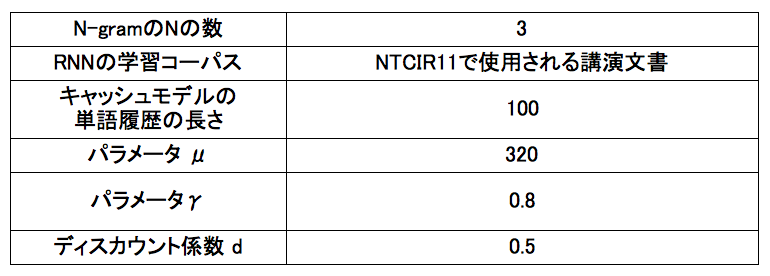
\includegraphics[width=7cm]{./image/t_feature1_2.png}
    \label{t_feture}
\end{table}

\subsection{実験結果}

% TODO: クエリ尤度のときの式を定義
実験を行った結果を表\ref{t_feture_res}に示す.

\begin{table}[h]
    \centering
    \caption{実験結果}
    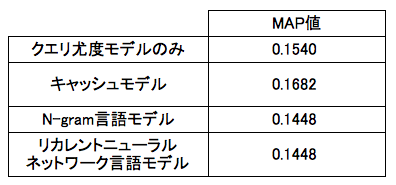
\includegraphics[width=7cm]{./image/t_feature2_1.png}
    \label{t_feture_res}
\end{table}

表\ref{t_feture_res}から,キャッシュモデルを適用したときに,MAP値の向上が見られた.しかし,N-gram言語モデルやリカレントニューラルネットワーク言語モデルを適用した場合に精度が低下した. 

% TODO: とても怪しい,アルゴリズムから見直した方が良い
本手法において,N-gram言語モデルは,検索対象の文書に対して学習を行なっている.NTCIR11 SpokenQuery\&Doc Formal-run の SQSCR SGS Retrieval条件では,検索対象文書が短いため,N-gram言語モデルが上手く学習できず,MAP値が低下したと考えられる.

また,リカレントニューラルネットワーク言語モデルは,講義単位で文脈を保持している.そのため,保持する情報が長過ぎることがMAP値の減少を引き起こしていると推察できる.キャッシュモデルにおいて,単語履歴の長さが長過ぎる場合に,MAP値が減少することが確認されており,リカレントニューラルネットワーク言語モデルも同様に,この現象が起こっていると考えられる.